\documentclass[8pt]{beamer}
\usepackage{pst-plot}
\usepackage[utf8]{inputenc}  
\usepackage[english, russian]{babel}
\usepackage{indentfirst}
\usepackage{graphicx}
\usepackage{pgf,pgfplots}
\usepackage{ragged2e}

\setbeamertemplate{caption}[numbered]
\setbeamertemplate{navigation symbols}{}

\usetheme{Singapore}
\title{Практикум на ЭВМ.\\ Отчет по четвертому заданию.}
\author{ Родин Иван, Сумин Даниил, Донской Иван\\ 311 группа}
\institute{Московский государственный университет им. Ломоносова}
\date{2018}

\begin{document}
 
\frame{\titlepage}
 
\begin{frame}
\frametitle{Постановка задачи}

Идет война с Семью Королевствами. Поставщики оружия стали не столь надежны, но времени терять нельзя. Нужно помочь Тириону Ланнистеру выбрать, с каким из поставщиков стали, Westeros Inc. или Harpy & Co., ему заключить договор о сотрудничестве.\\

\bigskip

С связи с этим, наша задача - проанализировать известные нам данные, из которых требуется сделать соответствующие выводы о качестве стали двух поставщиков, и решить, с каким из них было бы выгоднее заключить договор о закупке.\\
\end{frame}
 
\begin{frame}
\frametitle{Цель работы}
У нас есть данные о производстве мечей каждым из кузнецов и данные о количестве сломанных мечей в каждый из месяцев войны.

\bigskip

Нужно провести анализ этих данных, чтобы точно решить, с каким из кузнецов мы будем сотрудничать. Для этого мы сравнили модели по некоторым показателям
\end{frame}

\begin{frame}
\frametitle{Производство товара\\}
\begin{figure}[h]
\center{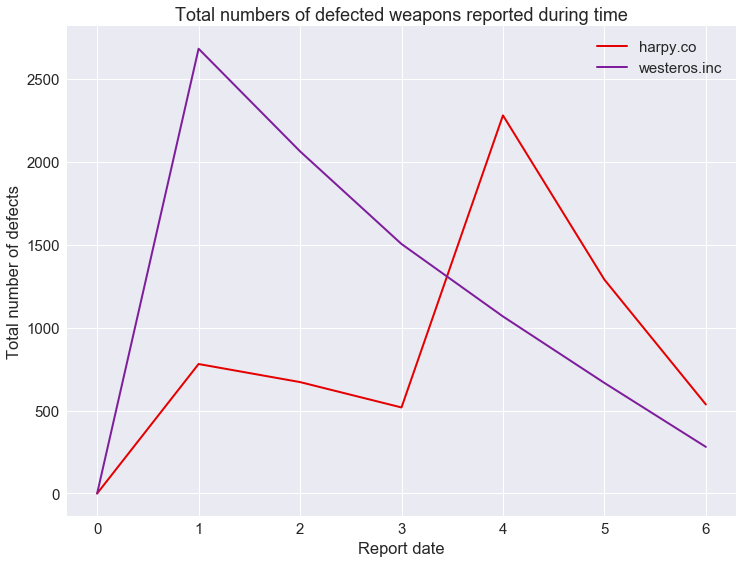
\includegraphics[width=1\linewidth]{img/4.jpg}}
\end{figure}
\bigskip
Мы видим, что обе компании поставляют примерно равное количество стали в каждый из месяцев, поэтому этот фактор не будет влиять на наш выбор


\end{frame}

\begin{frame}
\frametitle{Среднее нормированное число дефектов }
\begin{figure}[h]
\center{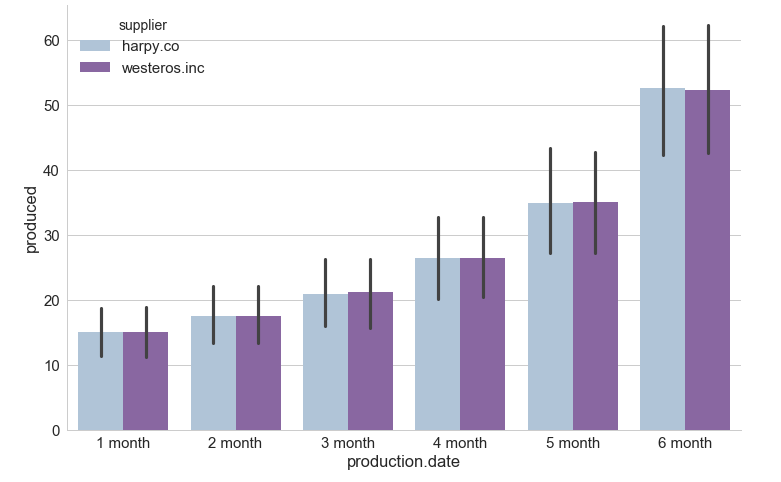
\includegraphics[width=0.93\linewidth]{img/3.jpg}}
\end{figure}
Представлен график, показывающий зависимость нормированного среднего числа дефектов от "возраста" оружия. Отметим, что информация о дефектах оружия "возраста" 6 месяцев встречается в 6 раз реже чем аналогичная информация о оружии "возраста" 1 месяц. Поэтому для адекватности сравнения была произведена нормировка.
Из графика видно, что в первые 3 месяца первая компания превосходит вторую, а в последующие 3 месяца - вторая

\end{frame}

\begin{frame}
\frametitle{Распределение дефектов }
\begin{figure}[h]
\center{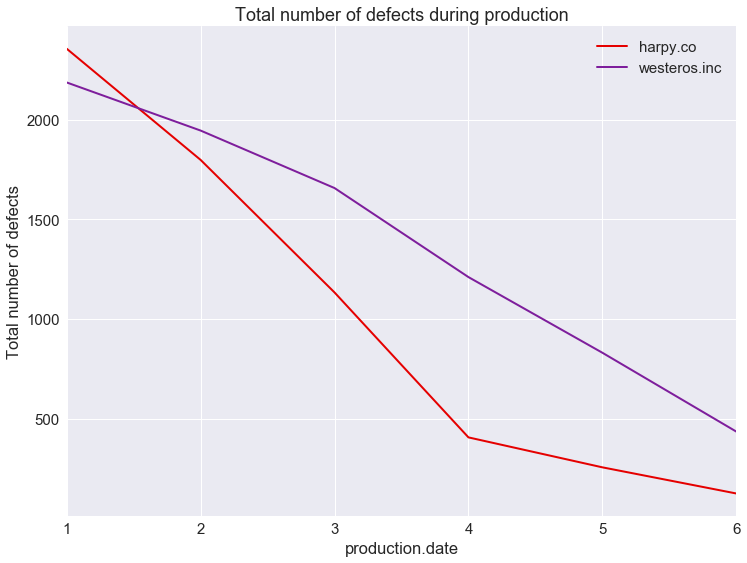
\includegraphics[width=0.92\linewidth]{img/6.jpg}}
\end{figure}
График показывает, какой процент от общего числа дефектов составляют дефекты оружия "возраста" x ( с учетом нормировки)
Из графика видно, что в первые 3 месяца оружие первой компании почти не ломается, затем происходит резкий скачок и оружие с высокой вероятностью сломается. У второй компании сразу наблюдается довольно высокий процент поломок, который равномерно уменьшается с "возрастом" оружия

\end{frame}



\begin{frame}

\frametitle{Модель для сравнения\\}
Для сравнения моделей построим некоторую простую модель. Сравним их с точки зрения пользы, которую принесет оружие до момента, пока не сломается. Будем считать, что оружие приносит 1 у.е. пользы за месяц использования, если оно не сломалось в этот месяц. Иначе будем полагать, что оружие принесло 0,5 у.е. Построим зависимость полученной пользы при взаимодействии с каждой компанией от срока использования стали


\end{frame}


\begin{frame}
\frametitle{Сравнение\\}
\begin{figure}[h]
\center{\includegraphics[width=1\linewidth]{img/model.jpg}}
\end{figure}
\bigskip
 Мы видим, что в рамках описанной модели больше пользы приносит сталь компании Harpy.co. При этом это выполняется для любого "возраста" оружия


\end{frame}


\begin{frame}
\frametitle{Общий процент сломанной продукции}
\begin{figure}[h]
\center{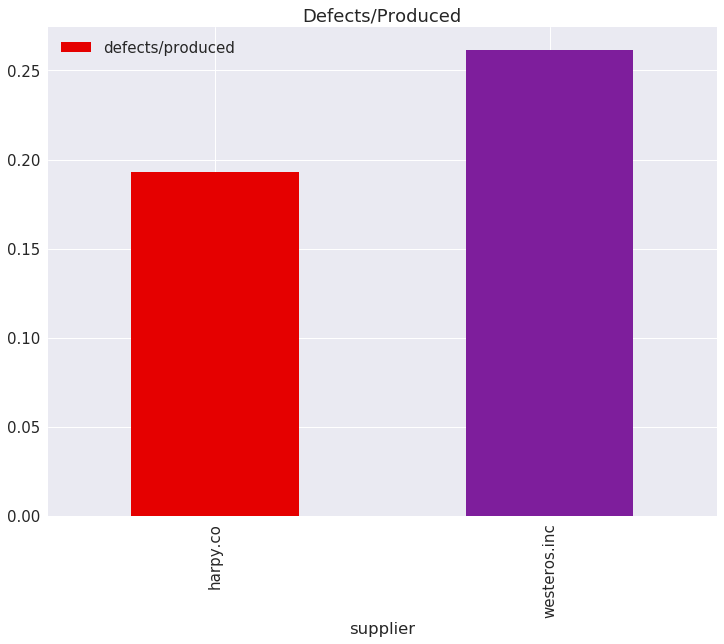
\includegraphics[width=0.8\linewidth]{img/2.jpg}}
\end{figure}
Возможно, влияет не только "возраст" оружия на поломки, но и текущий месяц?(погодные условия). Для этого построен график, показывающий процент сломанных мечей от количества мечей на данный момент. В рамках одной компании данные не очень полезны, так как с увеличением месяца увеличивается и количество более старых орудий. Но при этом мы можем сравнивать показатели двух производителей. Видно, что у Harpy.co в каждый календарный месяц меньше процент поломанных мечей, что очередной раз говорит в её пользу


\end{frame}
\begin{frame}
\frametitle{Выводы}
\begin{figure}[h]
\center{\includegraphics[width=1\linewidth]{img/dragons.jpg}}
\end{figure}
\bigskip
Исходя из всего вышесказанного, наша команда аналитиков решила посоветовать Тириону заключить договор с Harpy.co
\end{frame}



\end{document}